\chapter{Sistema Proposto}\label{cap_proposta}

{ O sistema proposto consiste em um \textit{soft-core} da \textit{ISA RISC-V}
    de 32 \textit{bits} com as extensões \textbf{I}, \textbf{M} e \textbf{F},
    podendo ser sintetizado nas versões \textit{RV32I}, \textit{RV32IM} ou
    \textit{RV32IMF}. A extensão \textit{Zicsr} com os Registradores de Controle
    e Estado (\textit{CSR}) é parcialmente implementada em todas as três
    configurações.
}

{ Cada uma das combinações da \textit{ISA} pode ser realizada em três
    microarquiteturas diferentes: unicicilo, multiciclo ou \textit{pipeline} de
    cinco estágios. Assim, o processador pode ser sintetizado em nove
    combinações diferentes.
}

{ O projeto utiliza a placa de desenvolvimento \textit{terasIC DE1-SoC} contendo
    diversos periféricos e um \textit{SoC Intel Altera Cyclone-V}. Vários dos
    periféricos presentes na plataforma tem controladores implementados com
    Entradas e Saídas Mapeadas em Memória (\textit{MMIO}) para que o
    \textit{soft-core} possa utilizá-los. A síntese dos controladores desses
    periféricos, como a saída de vídeo, entrada de teclado e barramento
    \textit{RS-232} é opcional.
}

{ O trabalho também é organizado de forma a facilitar a migração para placas de
    desenvolvimento diferentes da \textit{DE1-SoC} ou trocar o \textit{soft-core}
    desenvolvido por outra implementação, independente da sua \textit{ISA}.
    Todas as opções de configuração estão presentes em um único arquivo,
    centralizando as opções de customização do sistema gerado.
}


\section{Implementação da Microarquitetura Uniciclo}

    \begin{figure}[H]
    \centering
        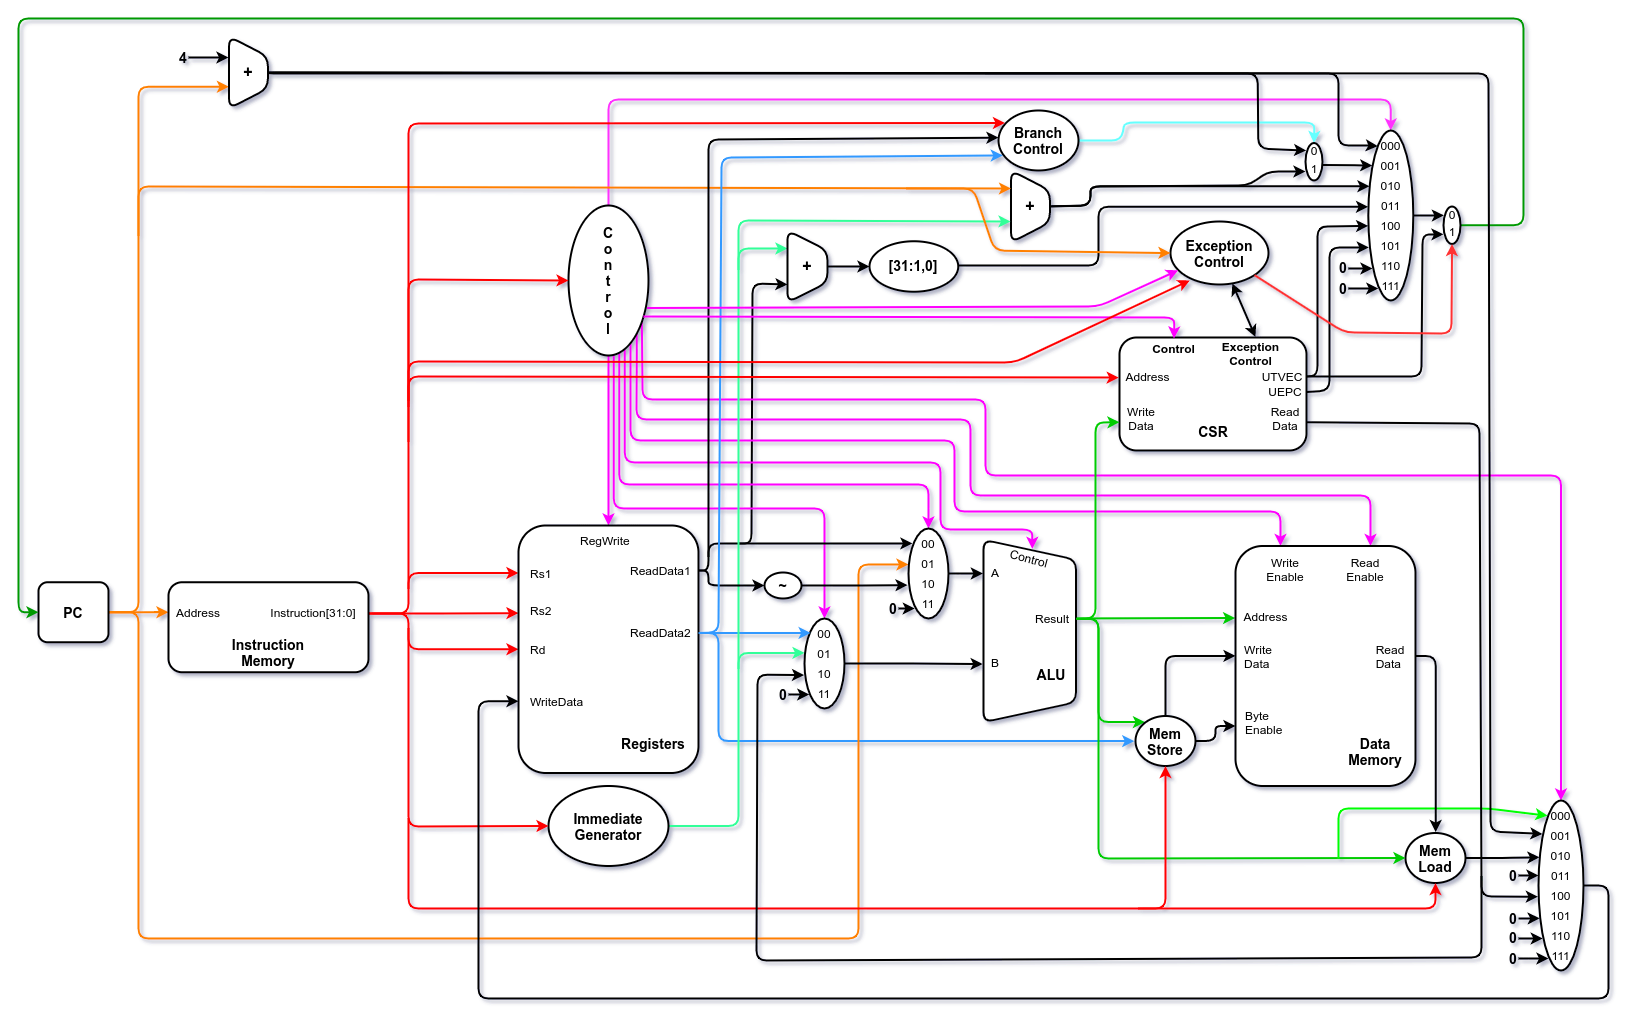
\includegraphics[width=1\linewidth]{../images/uarch_diagrams/singlecycle-RV32I-RV32IM.png}
        \caption{Diagrama da implementação das \textit{ISAs} RV32I e RV32IM na
        microarquitetura uniciclo.}\label{fig:diagram_rv32i_uni}
    \end{figure}

    \begin{figure}[H]
    \centering
        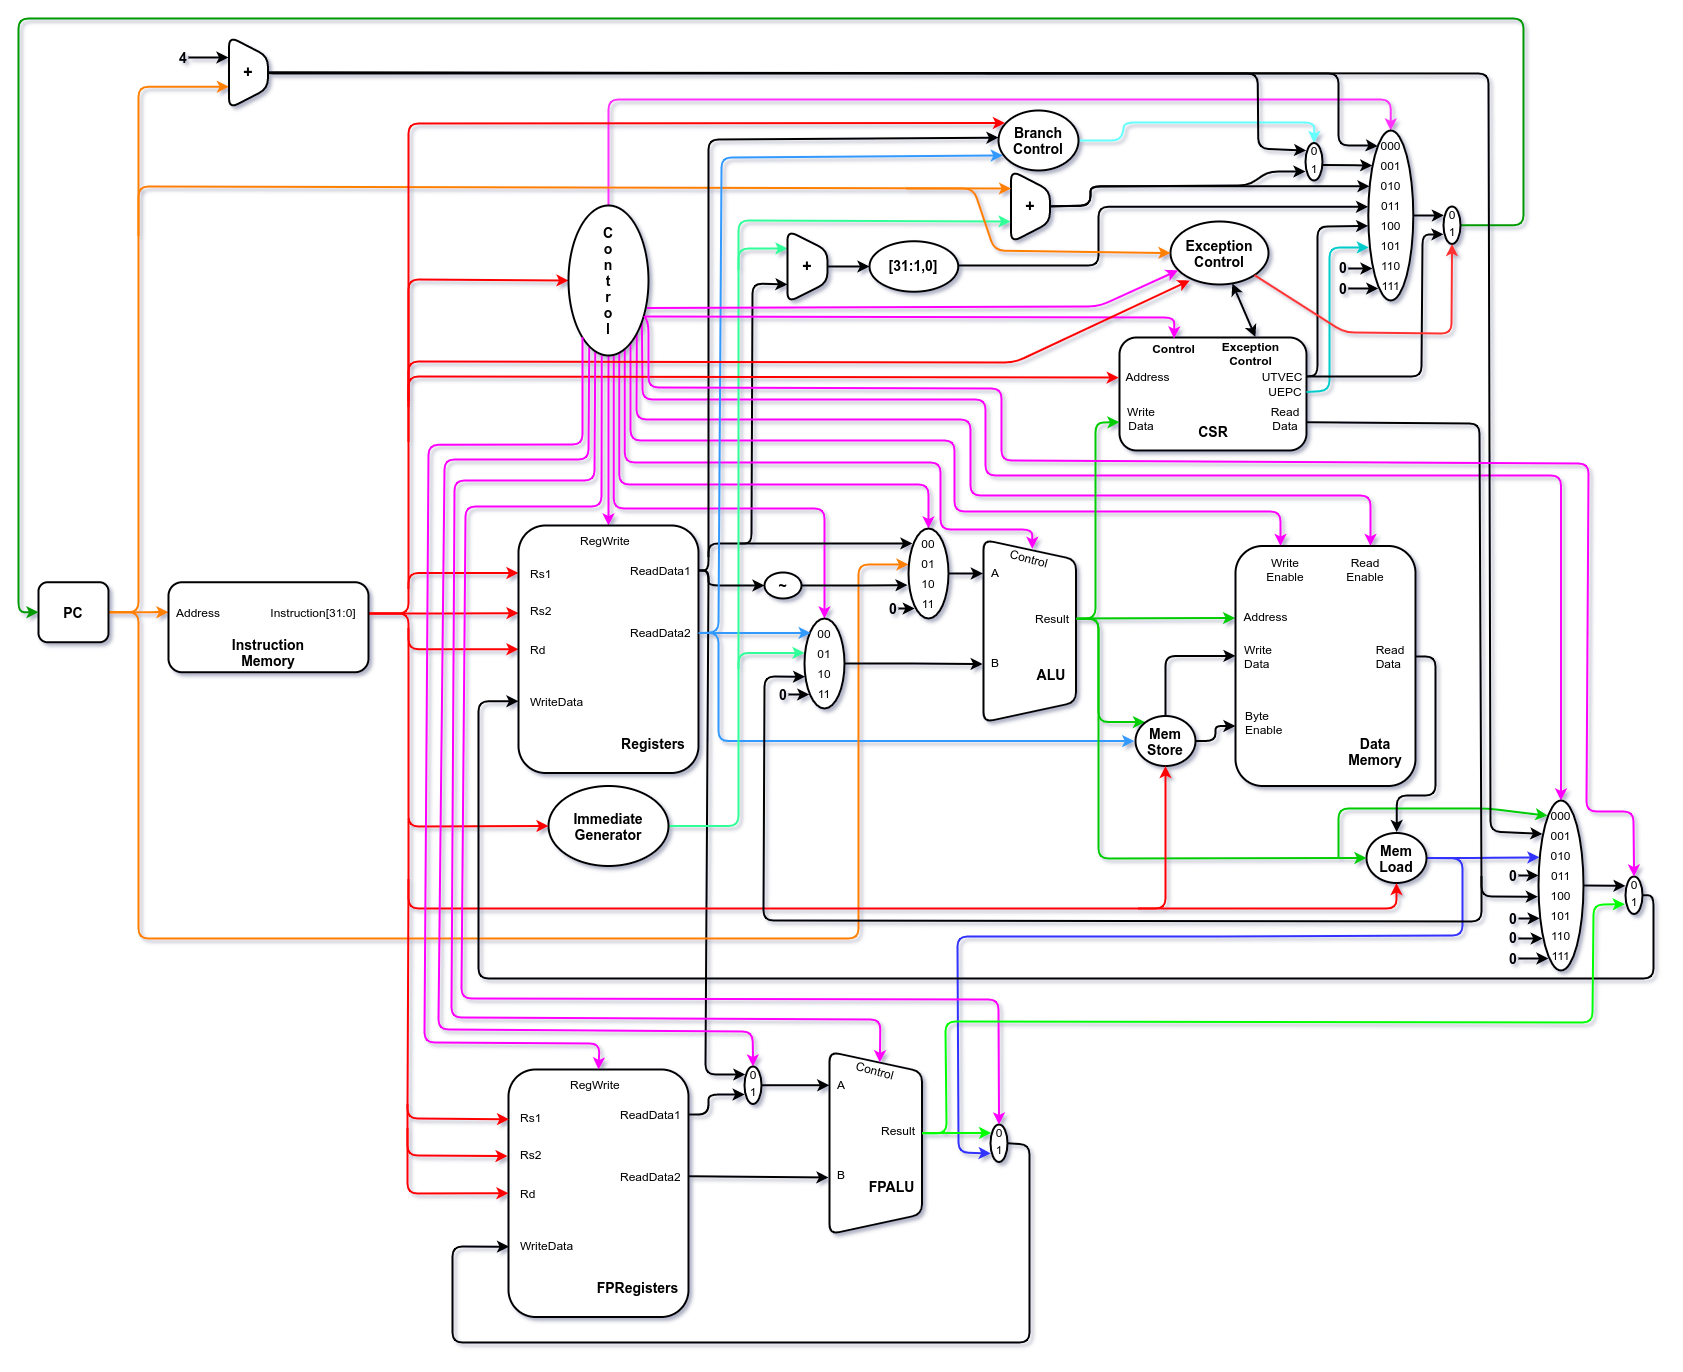
\includegraphics[width=1\linewidth]{../images/uarch_diagrams/singlecycle-RV32IMF.png}
        \caption{Diagrama da implementação da \textit{ISA} RV32IMF na
        microarquitetura uniciclo.}\label{fig:diagram_rv32imf_uni}
    \end{figure}

\section{Implementação da Microarquitetura Multiciclo}

    \begin{figure}[H]
    \centering
        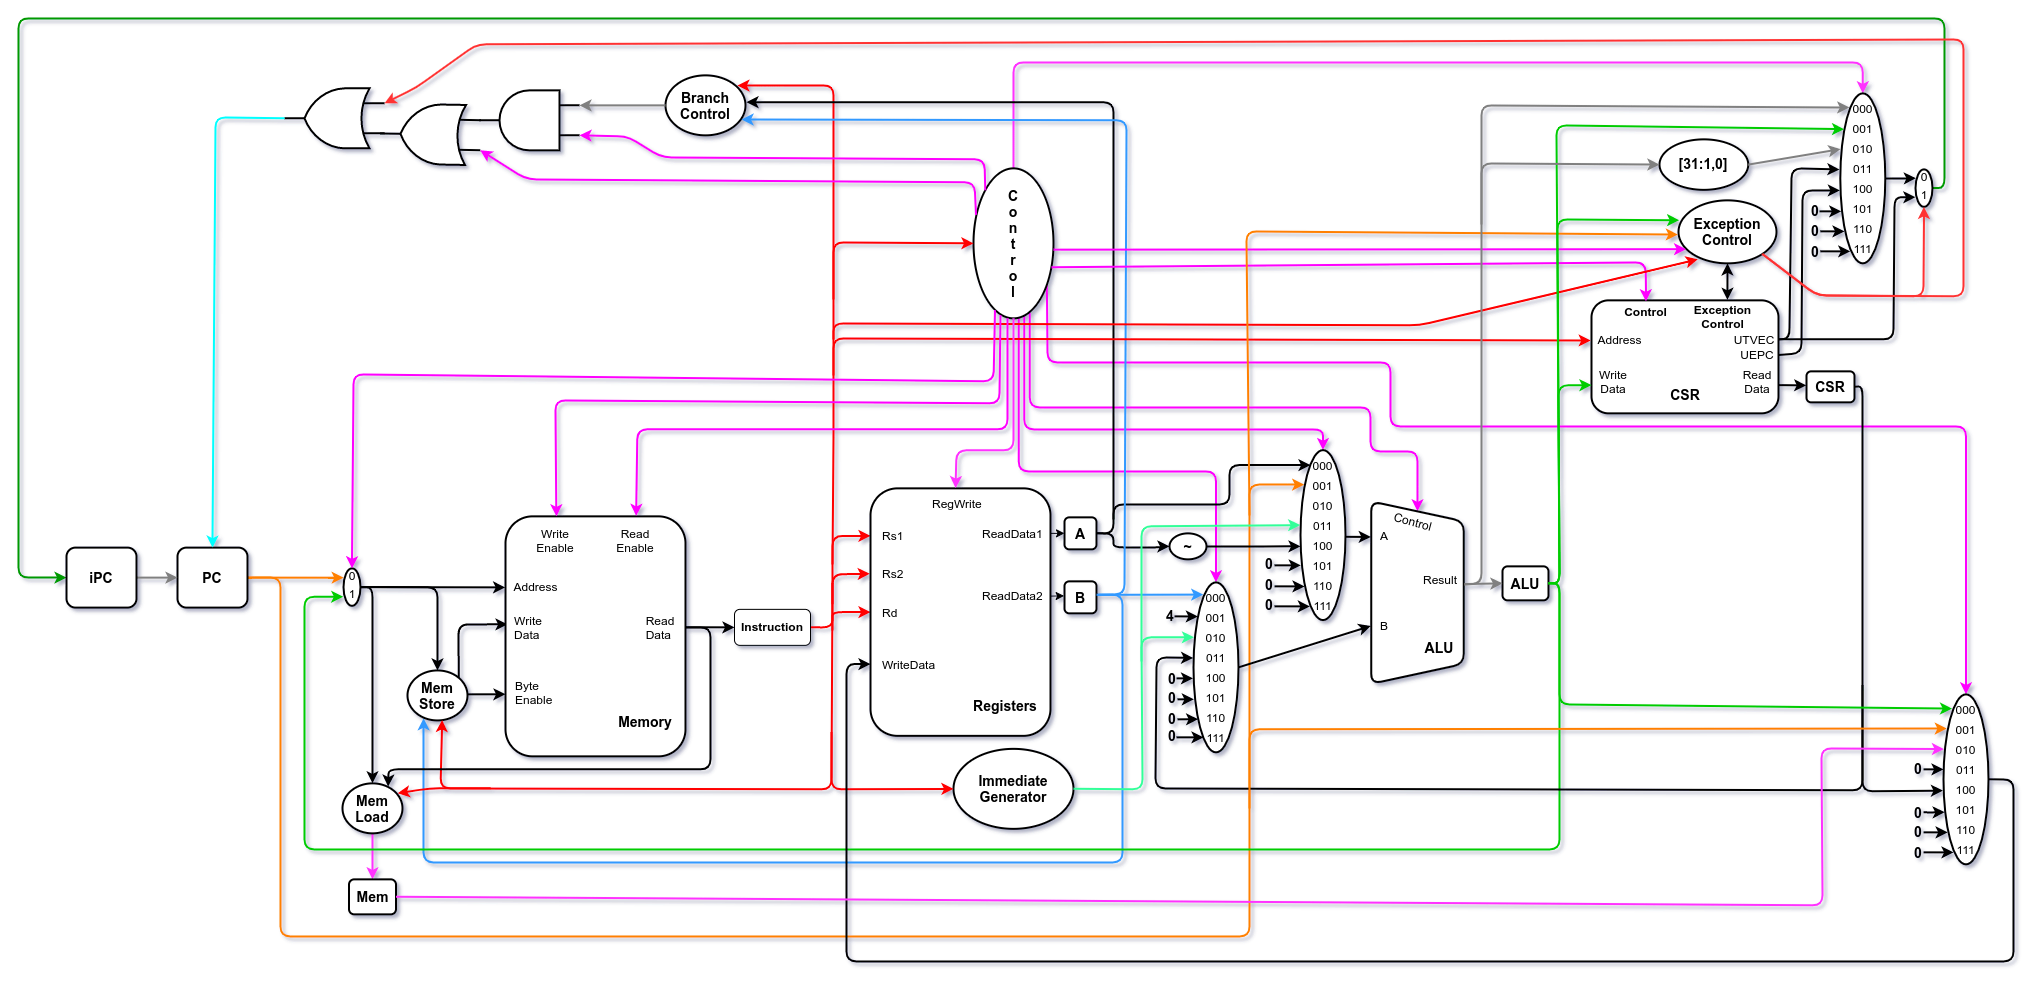
\includegraphics[width=1\linewidth]{../images/uarch_diagrams/multicycle-RV32I-RV32IM.png}
        \caption{Diagrama da implementação das \textit{ISAs} RV32I e RV32IM na
        microarquitetura multiciclo.}\label{fig:diagram_rv32i_multi}
    \end{figure}

    \begin{figure}[H]
    \centering
        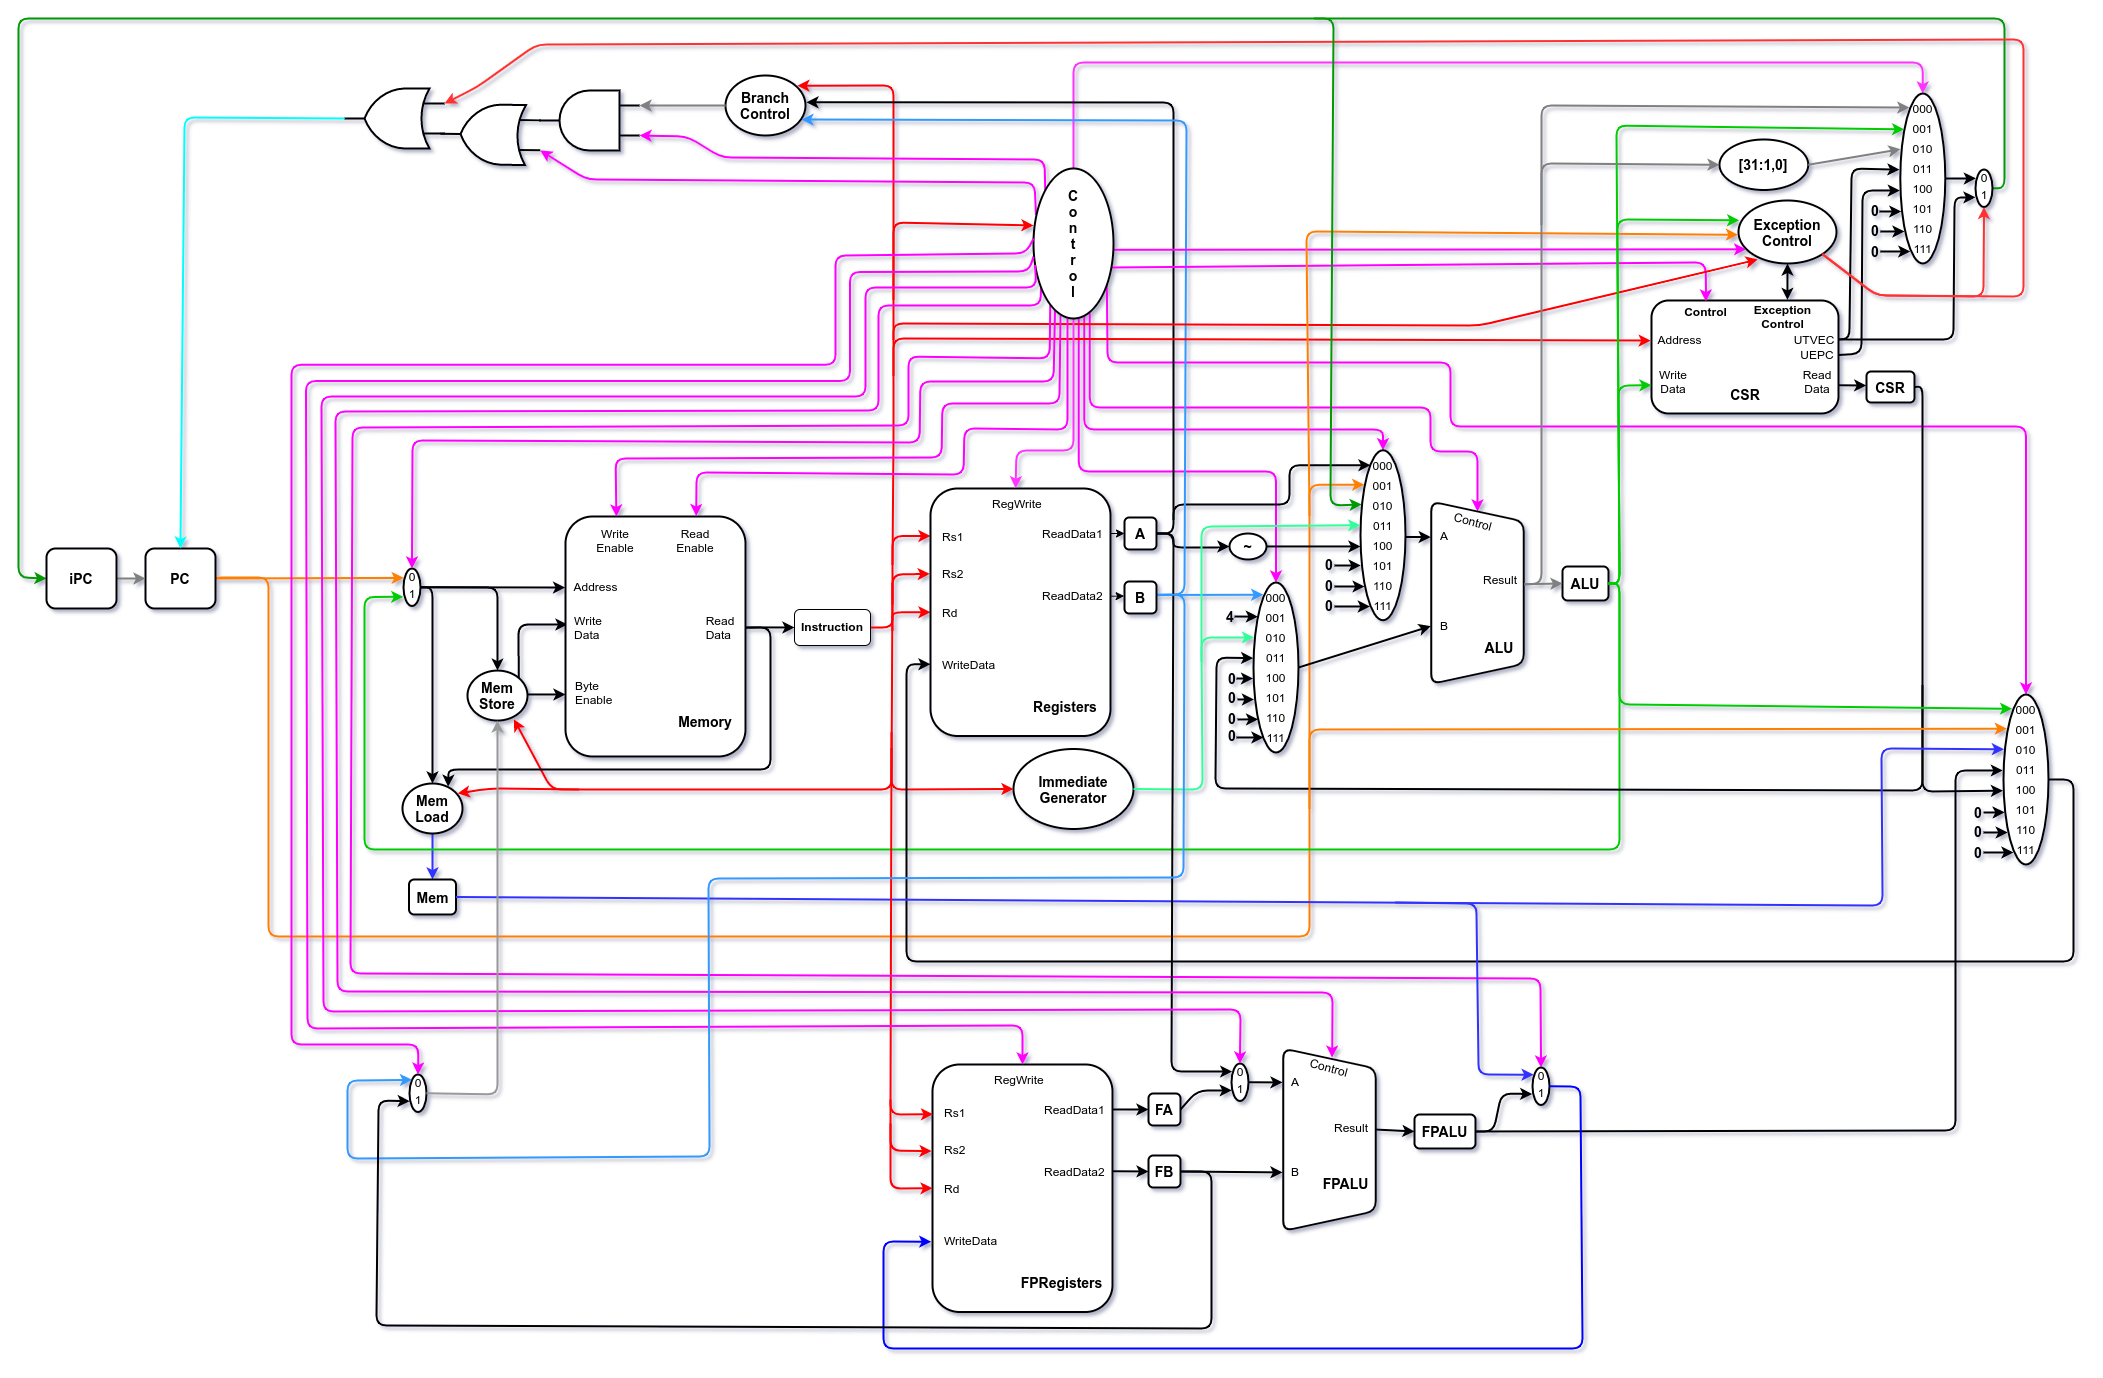
\includegraphics[width=1\linewidth]{../images/uarch_diagrams/multicycle-RV32IMF.png}
        \caption{Diagrama da implementação da \textit{ISA} RV32IMF na
        microarquitetura multiciclo.}\label{fig:diagram_rv32imf_multi}
    \end{figure}


\section{Implementação da Microarquitetura \textit{Pipeline} de 5 Estágios}

    \begin{figure}[H]
    \centering
        
\includegraphics[width=1\linewidth]{../images/placeholder.jpg}
        \caption{Diagrama da implementação das \textit{ISAs} RV32I e RV32IM na
        microarquitetura \textit{pipeline} de 5 estágios.}\label{fig:diagram_rv32i_pipe}
    \end{figure}

    \begin{figure}[H]
    \centering
        
\includegraphics[width=1\linewidth]{../images/placeholder.jpg}
        \caption{Diagrama da implementação da \textit{ISA} RV32IMF na
        microarquitetura \textit{pipeline} de 5 estágios.}\label{fig:diagram_rv32imf_pipe}
    \end{figure}





